\chapter{Военные корабли и их операторы}
\label{ch:ships-chapter}

Глава посвящена отечественным и зарубежным кораблям. Они могут иметь как военное, так и гражданское назначение. Гражданские суда используются в грузоперевозках, рыболовстве, туризме, разведке полезных ископаемых, спасательных работах, а также в спортивных, культурных и других целях. Для хранения информации о судах и других объектах ведутся базы знаний. Одной из таких баз знаний являются Викиданные. В этой главе изучены хранимые в Викиданных объекты кораблей и проведена оценка качества и полноты их описания.


\begin{marginfigure}[0.0cm]
  {
    \setlength{\fboxsep}{0pt}%
    \setlength{\fboxrule}{1pt}%
    \fcolorbox{gray}{gray}{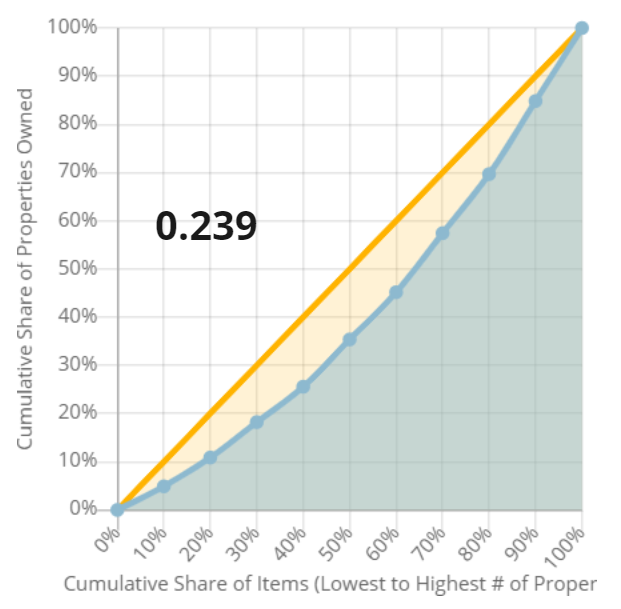
\includegraphics{chapter/ship/Russian_ships_topic_imbalance.png}}
  }
  \caption[График равномерности заполнения свойств объектов Викиданных.]{График равномерности заполнения по числу свойств объекта Викиданных \href{https://www.wikidata.org/wiki/Q11446}{корабль (Q11446)}, коэффициент Джини равен 0.239. Данные получены с помощью сервиса ProWD.id, 2020 год. График и коэффициент Джини показывают низкую равномерность заполнения свойств.}%
  \label{fig:prowd_ships-unbalanced}%
\end{marginfigure}


\section{Список кораблей}

\marginnote{
\href{https://www.wikidata.org/wiki/Q11446}{Корабль (Q11446)} -- это крупное морское судно.

Исследуемые свойства:
\begin{itemize}
  \item\href{https://www.wikidata.org/wiki/Property:P31}{Экземпляр (P31)};
  \item\href{https://www.wikidata.org/wiki/Property:P137}{Оператор (P137)};
  \item\href{https://www.wikidata.org/wiki/Property:P17}{Государство (P17)};
  \item\href{https://www.wikidata.org/wiki/Property:P607}{Конфликт (P607)}.
\end{itemize}
}

Построим список всех кораблей с помощью запроса~\ref{lst:ships_ru}.

\begin{lstlisting}[ language=SPARQL, caption={{\href{https://w.wiki/wX6}{Список кораблей}}\protect\footnotemark}, label=lst:ships_ru, ]
# List of ships
SELECT ?ship ?shipLabel
WHERE
{
  ?ship wdt:P31 wd:Q11446. # instance of ship
  SERVICE wikibase:label {bd:serviceParam wikibase:language "ru, en"}
}
\end{lstlisting}
\footnotetext{Найдено \num{19820} кораблей в 2017, \num{50681} в 2020, \num{71203} в 2021. Ссылка на SPARQL-запрос: \href{https://w.wiki/wX6}{https://w.wiki/wX6}}

По данным ProWD больше всего свойств (34 свойства) имеет \href{https://www.wikidata.org/wiki/Q281147}{ледокол Красин (Q281147)}, а меньше всего, по пять свойств, у кораблей \href{https://www.wikidata.org/wiki/Q99198666}{Ливень (Q99198666)} и \href{https://www.wikidata.org/wiki/Q28155282}{Dispatch (Q28155282)}~\autocite{ProWD_ru_ships}.

В Викиданных как правило записывается не прямая принадлежность корабля стране, а принадлежность некоторому оператору. Чаще всего это какая-либо организация, например, \href{https://www.wikidata.org/wiki/Q465283}{Военно-морской Флот Российской Федерации (Q465283)}. Составим список кораблей, операторы которых находятся или находились в России, СССР или Российской империи (см. листинг~\ref{lst:ships_with_ru_op}).

\begin{lstlisting}[ language=SPARQL, 
    caption={\href{https://w.wiki/3K$d}{Cписок кораблей, операторы которых находятся или находились в России, СССР или Российской Империи}\protect\footnotemark}, 
    label=lst:ships_with_ru_op 
                  ]
# List of ships from Russia, Soviet Union and Russian Empire
SELECT ?ship ?shipLabel
WHERE
{
  VALUES ?country {wd:Q34266 # Russian Empire
                   wd:Q15180 # Soviet Union
                   wd:Q159}  # Russia
  ?ship wdt:P31 wd:Q11446; # instance of ship
        wdt:P137/wdt:P17 ?country; # operator in country

  SERVICE wikibase:label {bd:serviceParam wikibase:language "ru, en"}
}
\end{lstlisting}
\footnotetext{Найдено 107 кораблей в 2017 году, 578 кораблей в 2021 году. Ссылка на SPARQL-запрос: \href{https://w.wiki/3K\%24d}{https://w.wiki/3K\$d}}


\section{Полнота Викиданных}

\label{question:ship_1}
\marginnote{Найдите <<корабль Гиннесса>> по какому-либо параметру. Например, напишите скрипт для поиска самого большого, самого длинного или самого вместительного корабля.\\ Ответ на странице~\pageref{answer:ship_Guinness}.}

Поиск точного количества кораблей в мире~--- трудная задача. 
Ведь данные о некоторых из них являются совершенно секретными, другие~--- частные судна и информации о них тоже нет. 
Предположим, что общее число кораблей примерно равно \num{1600000}, 
как указано в базе данных судов~\autocite{FleetMon}. 
На 2021 год Викиданные содержали только \num{71206} корабля, что составило только 4.5\% от их общего числа.


Что касается российских кораблей, в состав российский военных и гражданских флотов входит \num{17657} кораблей~\autocite{RussianShips}. В это же время скрипт в листинге~\ref{lst:ships_with_ru_op} показывает лишь 578 кораблей, что составляет 3.27\% от общего числа российских кораблей. 

В обоих случаях разница между фактическим количеством кораблей и результатом запросов огромная, что говорит о неполноте Викиданных.

\label{question:ship_2}
\marginnote{На рисунке~\ref{fig:grem_question} представлен самый известный советский эсминец \ruwiki{vgC}{проекта 7}, удостоенный звания <<Гвардейский>>, назовите его.  Ответ можно найти на странице~\pageref{answer:ship_2}.}

\begin{marginfigure}[0.0cm]
  {
    \setlength{\fboxsep}{0pt}%
    \setlength{\fboxrule}{1pt}%
    \fcolorbox{gray}{gray}{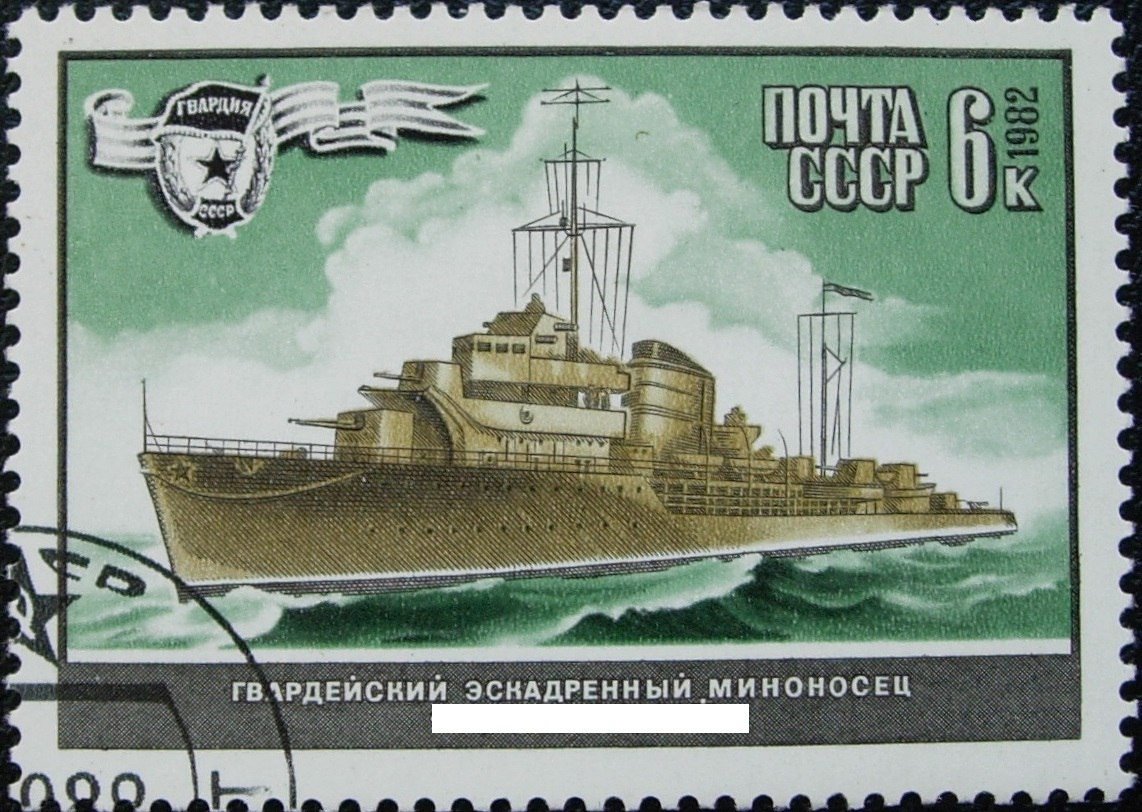
\includegraphics{chapter/ship/Secret_Grem_ship.jpg}}
  }
  \caption[Известный советский миноносец.]{Почтовая марка, на которой изображен известный советский \ruwiki{vgD}{эскадренный миноносец} \ruwiki{vgC}{проекта 7}, CCCP, 1982.}%
  \label{fig:grem_question}%
\end{marginfigure}

\section{Полнота свойств объектов военных кораблей}

Составим список кораблей, участвовавших в каких-либо конфликтах с помощью скрипта в листинге~\ref{lst:ships_in_conflict_ru}.

\begin{lstlisting}[ language=SPARQL, caption={{\href{https://w.wiki/vum}{Список кораблей, участвовавших в каких-либо конфликтах}}\protect\footnotemark}, label=lst:ships_in_conflict_ru, ]
# List of ships with countries and war conflicts
SELECT ?ship ?shipLabel ?countryLabel ?conflict ?conflictLabel
WHERE
{
  ?ship wdt:P31 wd:Q11446;        # instance of ship
        wdt:P137/wdt:P17 ?country;# belongs to country
        wdt:P607 ?conflict.       # engaged in some conflict
  SERVICE wikibase:label { bd:serviceParam wikibase:language "ru, en" }
}
\end{lstlisting}
\footnotetext{Найдено \num{1400} кораблей в 2017 году, \num{3567} в 2021 году. Ссылка на SPARQL-запрос: \href{https://w.wiki/vum}{https://w.wiki/vum}}

У военных кораблей, участвовавших в сражениях, указывается свойство \href{https://www.wikidata.org/wiki/Property:P607}{conflict (P607)} (война/сражение). В то же время военные конфликты и военные операции, которые являются частью войн, являются разными понятиями. Корабли на Викиданных можно условно по делить на два типа:

\begin{enumerate}
  \item Корабли, у которых военные операции объединены с военными конфликтами. Например, у \href{https://www.wikidata.org/wiki/Q4148613}{эсминца Гремящий (Q4148613)} 10 войн/сражений, см. листинг~\ref{lst:grem_wars}. Такое большое число связано с тем, что корабль принял участие во многих \href{https://ru.wikipedia.org/wiki/Арктические_конвои}{арктических конвоях}, которые являются военными операциями.
  \item Корабли, у которых военные операции отделены от военных конфликтов. Например, у британского крейсера \href{https://www.wikidata.org/wiki/Q1565575}{HMS Trinidad (Q1565575)} участие в военной кампании и арктическом конвое указаны как часть Второй мировой войны с помощью квалификатора \href{https://www.wikidata.org/wiki/Property:P1012}{including (P1012)}. Таким образом, в Викиданных у этого крейсера указана одна война/сражение.
\end{enumerate}

У кораблей первого типа при поиске по свойству~\wdProperty{607}{conflict} будет отображаться больше войн/сражений, чем у кораблей второго типа. 
%Но в этом случае операция \href{https://ru.wikipedia.org/wiki/Одесская_оборона_(1941)}{Одесская оборона} будет стоять наряду с \href{https://ru.wikipedia.org/wiki/Великая_Отечественная_война}{Великой Отечественной войной}, хотя она является частью этой войны. В такой ситуации выводимые данные будут не точными.

\label{question:ship_3}
\marginnote{Найдите изображения кораблей, заснятых в кино или описанных в книгах. 

Ответ на странице~\pageref{answer:ship_3}}


\begin{lstlisting}[ language=SPARQL, caption={{\href{https://w.wiki/vuo}{Военные конфликты, в которых участвовали \href{https://www.wikidata.org/wiki/Q4148613}{эсминец Гремящий (Q4148613)} и \href{https://www.wikidata.org/wiki/Q1565575}{HMS Trinidad (Q1565575)}}}\protect\footnotemark}, label=lst:grem_wars, ]
# List of military conflicts of the two ships 
SELECT ?ship ?shipLabel ?conflict ?conflictLabel
WHERE
{
  VALUES ?ship {wd:Q4148613   # Soviet destroyer Gremyashchiy
                wd:Q1565575}  # United Kingdom's HMS Trinidad
  ?ship wdt:P607 ?conflict.   # conflict
  SERVICE wikibase:label { bd:serviceParam wikibase:language "ru, en" }
}
\end{lstlisting}
\footnotetext{Найдено \num{10} конфликтов у \href{https://www.wikidata.org/wiki/Q4148613}{эсминца Гремящий (Q4148613)} и один конфликт у крейсера \href{https://www.wikidata.org/wiki/Q1565575}{HMS Trinidad (Q1565575)}, 2021 год. Ссылка на SPARQL-запрос: \href{https://w.wiki/vuo}{https://w.wiki/vuo}}

Составим список отечественных кораблей, участвовавших в каких-либо военных конфликтах с помощью скрипта~\ref{lst:ships_in_war_ru}.

\begin{lstlisting}[ language=SPARQL, 
        caption={{\href{https://w.wiki/wXA}{Список отечественных кораблей, участвовавших в каких-либо военных конфликтах}}\protect\footnotemark}, 
        label=lst:ships_in_war_ru ]
# List of ship with countries and war conflicts
SELECT ?ship ?shipLabel ?countryLabel ?conflict ?conflictLabel
WHERE
{
  VALUES ?country {wd:Q34266 # Russian Empire
                   wd:Q15180 # Soviet Union
                   wd:Q159}  # Russia
  ?ship wdt:P31 wd:Q11446;        # instance of ship
        wdt:P137/wdt:P17 ?country;# belongs to operator
        wdt:P607 ?conflict.       # engaged in some conflict

  SERVICE wikibase:label { bd:serviceParam wikibase:language "ru, en" }
}
\end{lstlisting}
\footnotetext{Найдено \num{105} кораблей в 2017 году, \num{82} корабля в 2021 году. Ссылка на SPARQL-запрос: \href{https://w.wiki/wXA}{https://w.wiki/wXA}}

Особенность результатов скрипта~\ref{lst:ships_in_war_ru} в том, 
что полученные корабли не обязательно связаны только с Российской империей, 
СССР или Россией. 
Например, корабль \href{https://www.wikidata.org/wiki/Q653477}{Kasato Maru (Q653477)}~--- японский. 
Дело в том, что этот корабль принадлежал России в 1900--1905 годы, а Японии с 1906 года.


\section{Корабли-музеи в странах мира}

\href{https://www.wikidata.org/wiki/Q575727}{Корабль-музей (Q575727)} это корабль, на котором размещена музейная экспозиция, посвященная истории корабля. Такие корабли используются в общеобразовательных и мемориальных целях. Участие корабля в \href{https://www.wikidata.org/wiki/Q180684}{военном конфликте (Q180684)} может послужить поводом для создания корабля-музея в память о прошедших событиях. 

Построим граф кораблей-музеев и стран, в которых эти корабли находятся. Вершинами графа будут \href{https://www.wikidata.org/wiki/Q6256}{страны (Q6256)} и \href{https://www.wikidata.org/wiki/Q575727}{корабли-музеи (Q575727)}. Ребро между кораблем и страной означает, что корабль находится в этой стране. А ребро между двумя странами означает, что эти страны участвовали в одних и тех же конфликтах, число которых равно весу ребра. Скрипт в листинге~\ref{lst:museum_graph} строит граф по описанным выше правилам.

%\begin{minipage}{\linewidth}
\begin{lstlisting}[ language=SPARQL, 
        caption={{\href{https://w.wiki/wz8}{Граф кораблей-музеев и стран, в которых они находятся (фрагмент скрипта)}}\protect\footnotemark}, 
        label=lst:museum_graph ]
#defaultView:Graph
SELECT ?v1 ?v1Label ?v2 ?v2Label ?edgeLabel ?img
WHERE {
  {SELECT ?c ?cLabel ?v1 ?v1Label ?v2 ?v2Label 
                 (STR(COUNT(?c)) as ?edgeLabel) 
    WHERE
    {
      . . .
      ?c wdt:P31 ?cTypes.   # ?c is war / conflict
      ?v1 wdt:P31 wd:Q6256. # v1 is country
      ?v2 wdt:P31 wd:Q6256. # v2 is country
      ?c wdt:P710 ?v1, ?v2. # v1 and v2 participated in war ?c
      FILTER (?v1 != ?v2 && STR(?v1) < STR(?v2)) 
      . . .
    }
    GROUP BY ?c ?cLabel ?v1 ?v1Label ?v2 ?v2Label
  }
  . . .
}
\end{lstlisting}
%\end{minipage}
\footnotetext{Найдено 117 вершин графа в 2021 году. Ссылка на SPARQL-запрос: \href{https://w.wiki/wz8}{https://w.wiki/wz8}.}
\marginnote[-7.3cm]{%
    При определении \wdqName{страны}{6256} для переменных $v1$ и $v2$ 
    используется конструкция ``p:/ps:''.
    Это нужно потому, что у стран в поле 
    \href{https://www.wikidata.org/wiki/Property:P31}{экземпляр (P31)}
    кроме значения <<страна>> могут быть и другие значения. 
    Конструкция ``p:/ps:'' позволяет перебрать все значения поля P31 и найти значение <<страна>>.
    См. подробности в главе~\ref{ch:RussiaNotCountryPPS} на странице~\pageref{ch:RussiaNotCountryPPS}.}
\marginnote[-1.7cm]{%
    Функция FILTER позволяет избежать появления петель и дублирующих рёбер на графе.
}

Из фрагмента графа на рисунке~\ref{fig:museum_graph} видно, 
что корабли-музеи по большей части принадлежат Германии, США и Японии. 
Такая <<корреляция>> вполне логична, так как данные страны имеют длительную историю, 
за которую они поучаствовали во многих военных конфликтах. 
Также эти страны имеют выход к морю, что исторически обуславливает наличие у них флота, 
в котором могут найтись корабли для создания музея.

\begin{figure*}[h]
  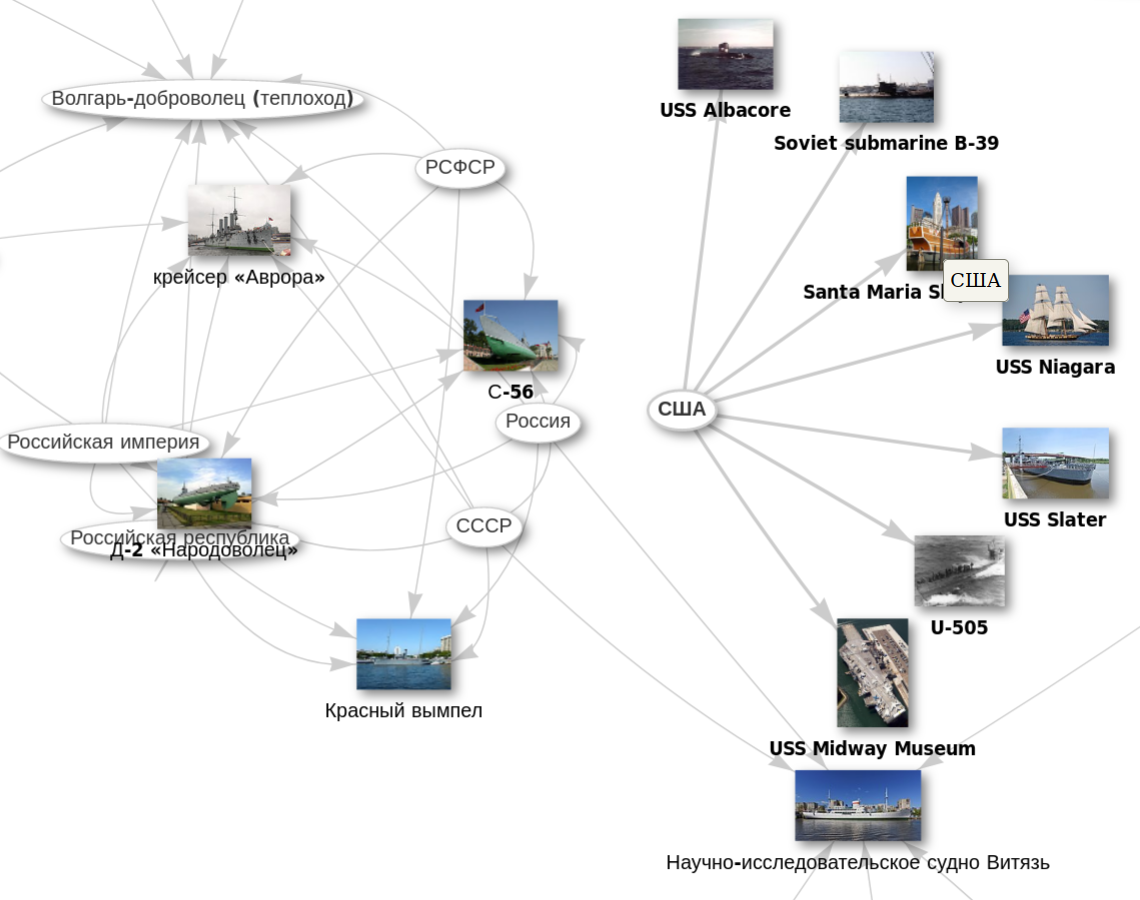
\includegraphics[width=0.8\linewidth]{chapter/ship/museum-graph-Russia-USA.png}
  \caption[Граф стран и кораблей-музеев, 2021 год.]{Фрагмент графа стран, участвовавших в войнах. Фрагмент включает ряд кораблей-музеев России и США. Граф построен по скрипту~\protect\ref{lst:museum_graph} в 2021 году.}%
  \label{fig:museum_graph}%
\end{figure*}

При просмотре полного графа (и даже на фрагменте, рис.~\ref{fig:museum_graph}) 
видно уникальность научно-исследовательского судна \wdqName{Витязь}{1516653}. 
По Викиданным (листинг~\ref{lst:museum_graph}), 
это единственный музей-корабль России, связывающий Россию с другими странами. 
Изначально этот теплоход был построен и находился на службе Германии, 
что отражено в свойстве Витязя 
\href{https://www.wikidata.org/wiki/Property:P137}{operator (P137)}=``Кригсмарине'', 
это название военно-морских сил в Третьем рейхе.

Вершины графа на рисунке~\ref{fig:museum_graph} кликабельны. Например, можно кликнуть на \href{https://www.wikidata.org/wiki/Q168713}{крейсер Аврора (Q168713)}, тогда появятся дополнительные вершины, соответствующие свойствам этого крейсера, см. рисунок~\ref{fig:aurora_graph}.

\newpage
\begin{figure*}[h]
  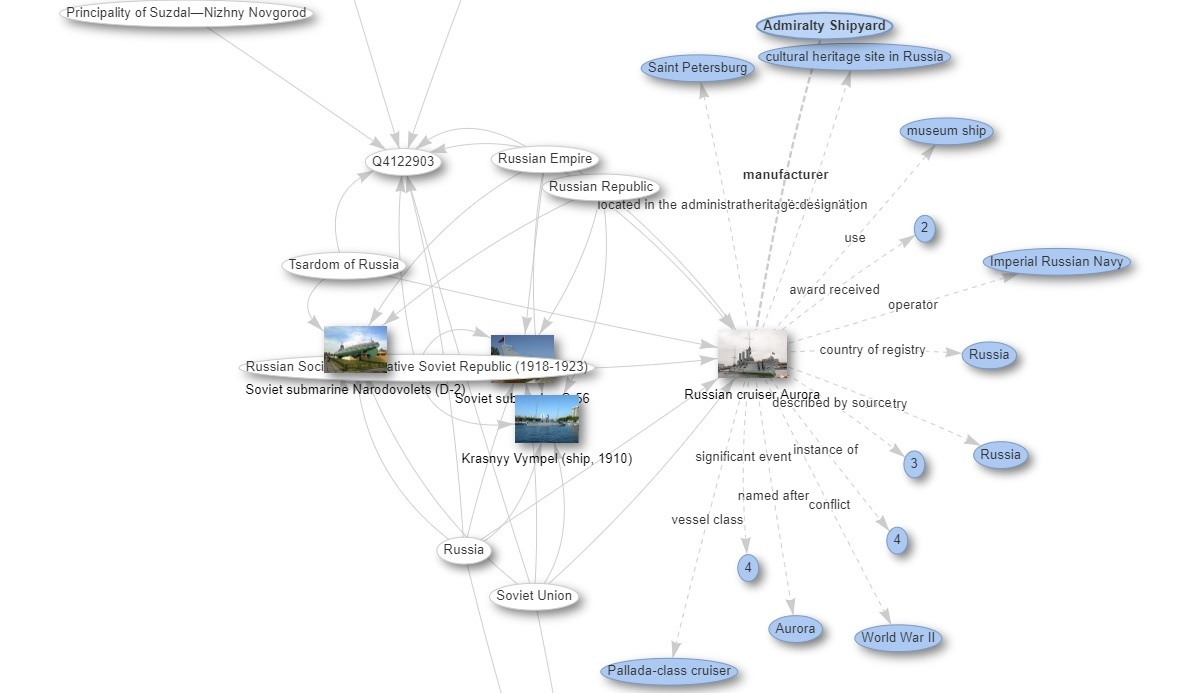
\includegraphics[width=\linewidth]{chapter/ship/aurora_graph.jpg}
  \caption[Граф свойств Авроры, 2021 год.]{Граф свойств \href{https://www.wikidata.org/wiki/Q168713}{крейсера Аврора (Q168713)} на 2021 год.}%
  \label{fig:aurora_graph}%
\end{figure*}






% last figure
%\begin{figure*}[ht]
%  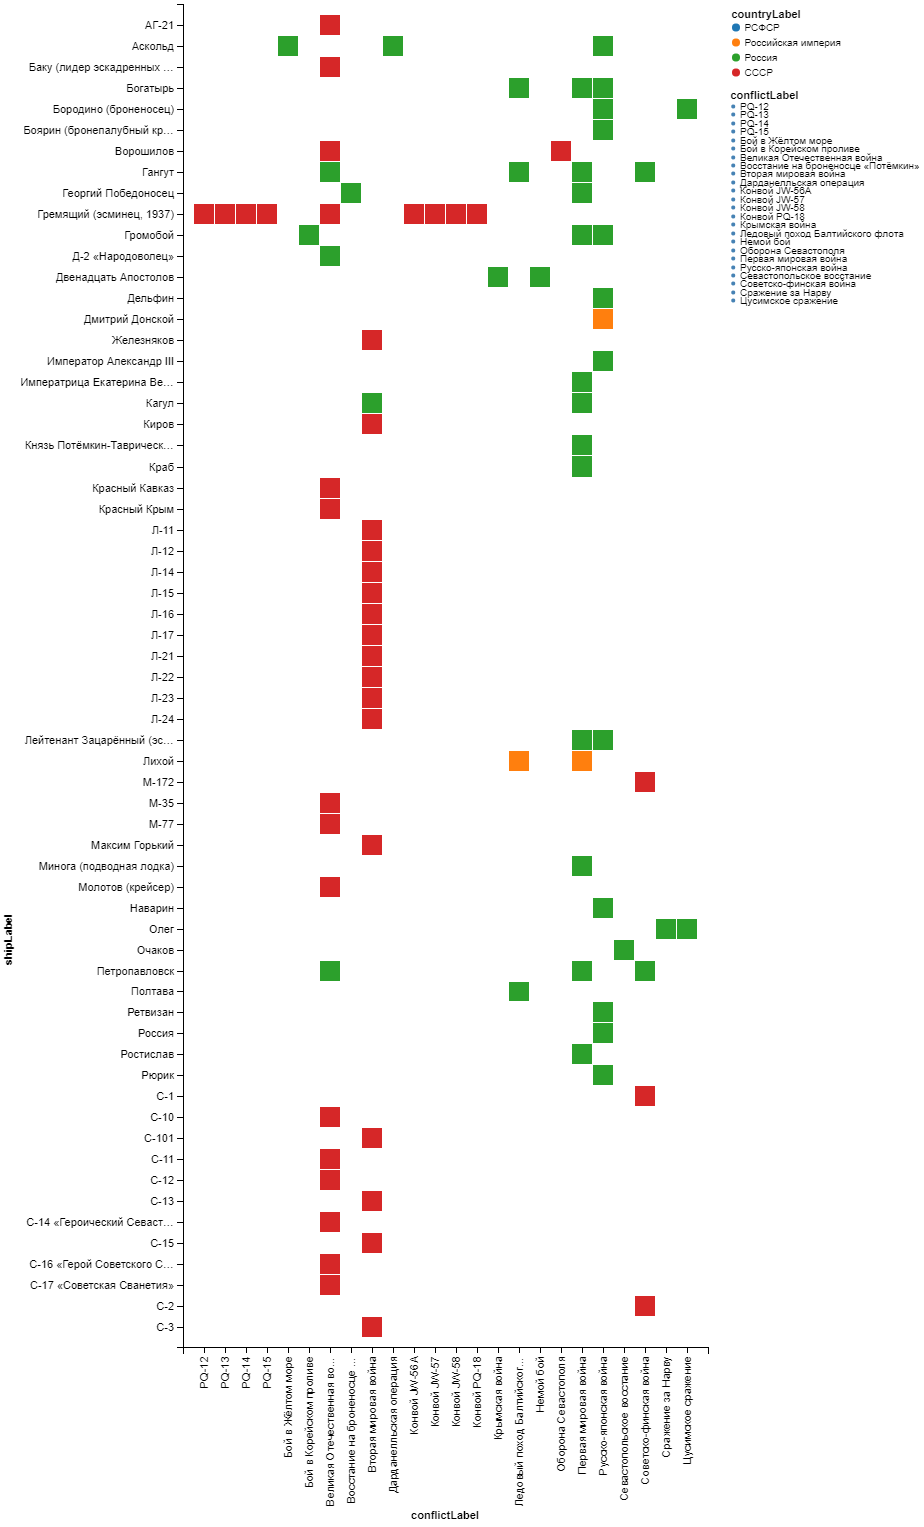
\includegraphics[width=0.25\linewidth]{chapter/ship/red-green-cells_ships_by_country_and_conflict.png}
%  \caption[Список кораблей и конфликтов, в которых они участвовали]{Фрагмент cписка кораблей, связанных с Россией и участвовавших в военных конфликтах, 2017 год. Из списка видно, что больше большая часть кораблей связаны с Россией и СССР, а также со Второй мировой или Великой Отечественной войнами.}%
%  \label{fig:ships_by_country_and_conflict}%
%\end{figure*}
